\chapter{Graphs}

A \emph{graph} is an ordered pair $G=(V,E)$ where $V$ is a set of
\emph{vertices} and $E$ is a set of \emph{edges}.  An edge is a pair
of vertices which are said to be \emph{adjacent}.  Usually we consider
edges to be unordered, in which case the graph is undirected and an
edge $\{A,B\}$ connects $A$ to $B$ and $B$ to $A$.  For example:

\begin{align*} 
V &= \{ A, B, C \} \\ E &= \{ (A, B), (B, C) \} 
\end{align*}

Which can be represented more visually:

{
  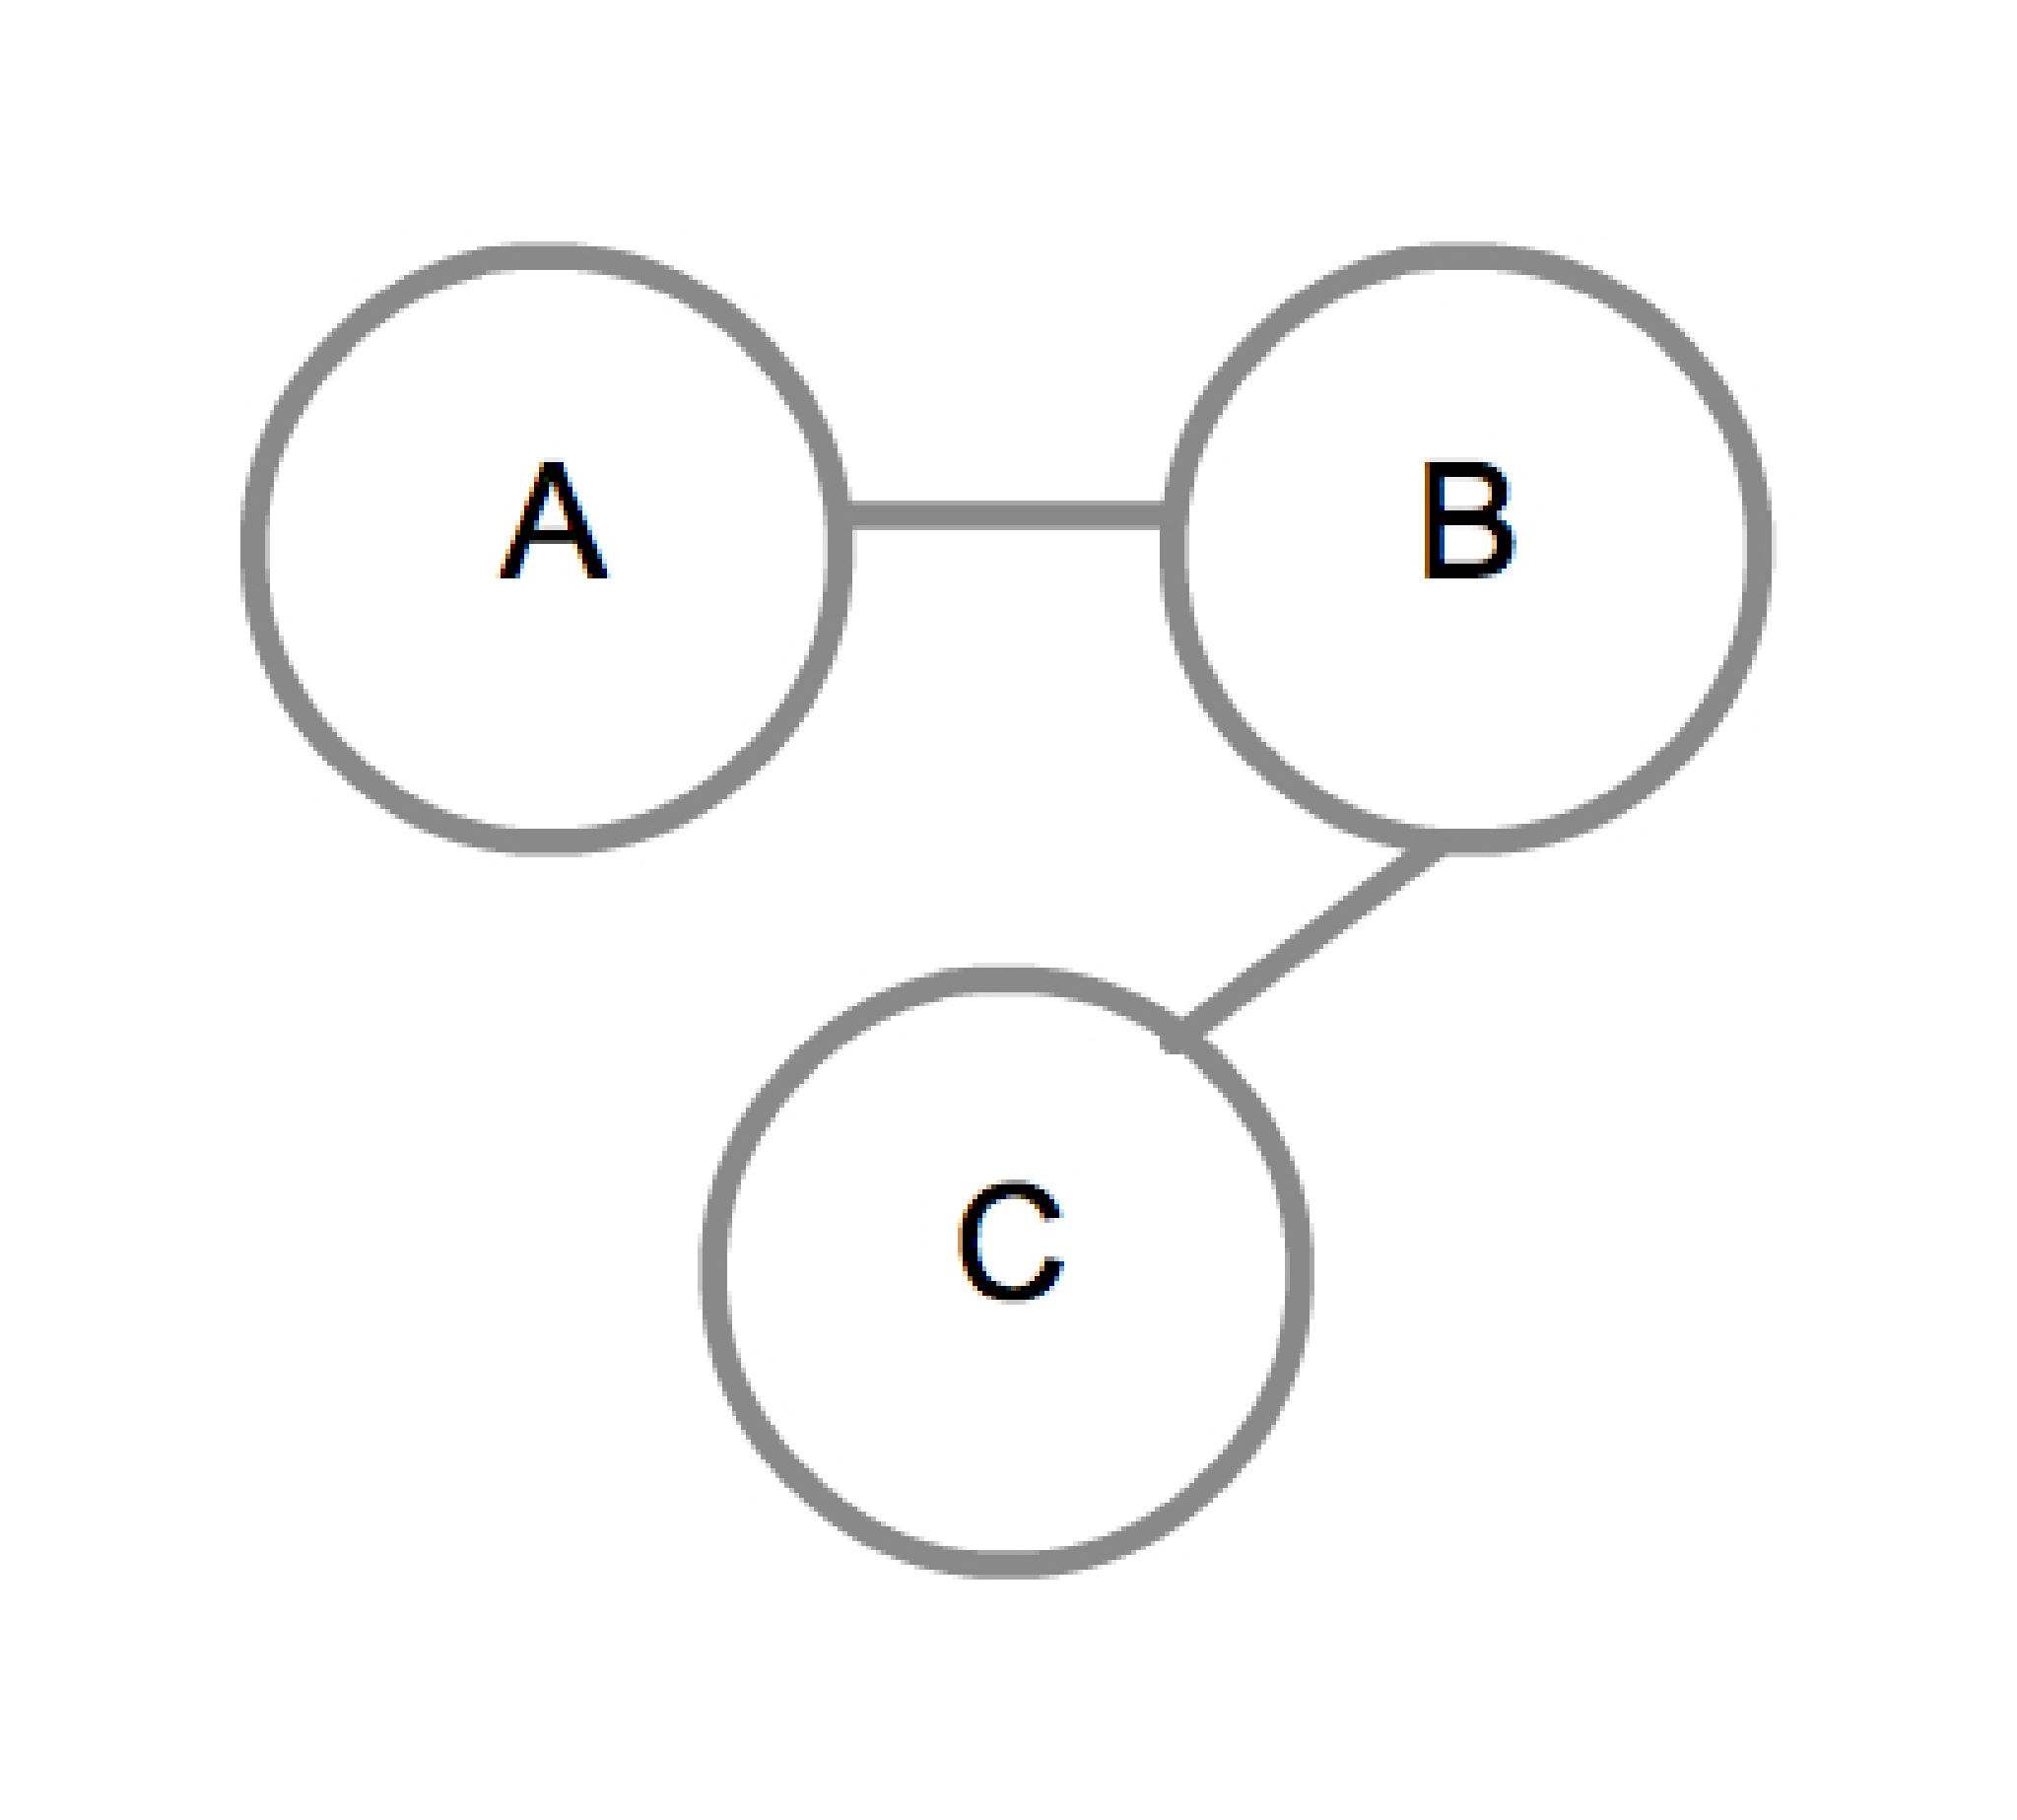
\includegraphics[scale=0.2]{SimpleGraph}
  %\caption{Demonstrates a simple graph}
  \label{fig:SimpleGraph}
}

Note that the vertices are represented by labeled circles and the
edges are represented by lines connecting vertices to one another.

The number of edges connecting a vertex $v$ is called the degree of
$v$ or $deg(v)$.  In the above example:

\begin{align*}
deg(A) = deg(C) &= 1 \\
deg(B) &= 2
\end{align*}

Sometimes an edge is directional, meaning the pair of vertices in an
edge is ordered.  In other words, the edge $(A, B)$ connects $A$ to
$B$, but not $B$ to $A$.  We say such an edge is incoming on $B$ and
outgoing on $A$.  This is represented visually by an edge with an
arrow at one end, indicating the direction:

{
  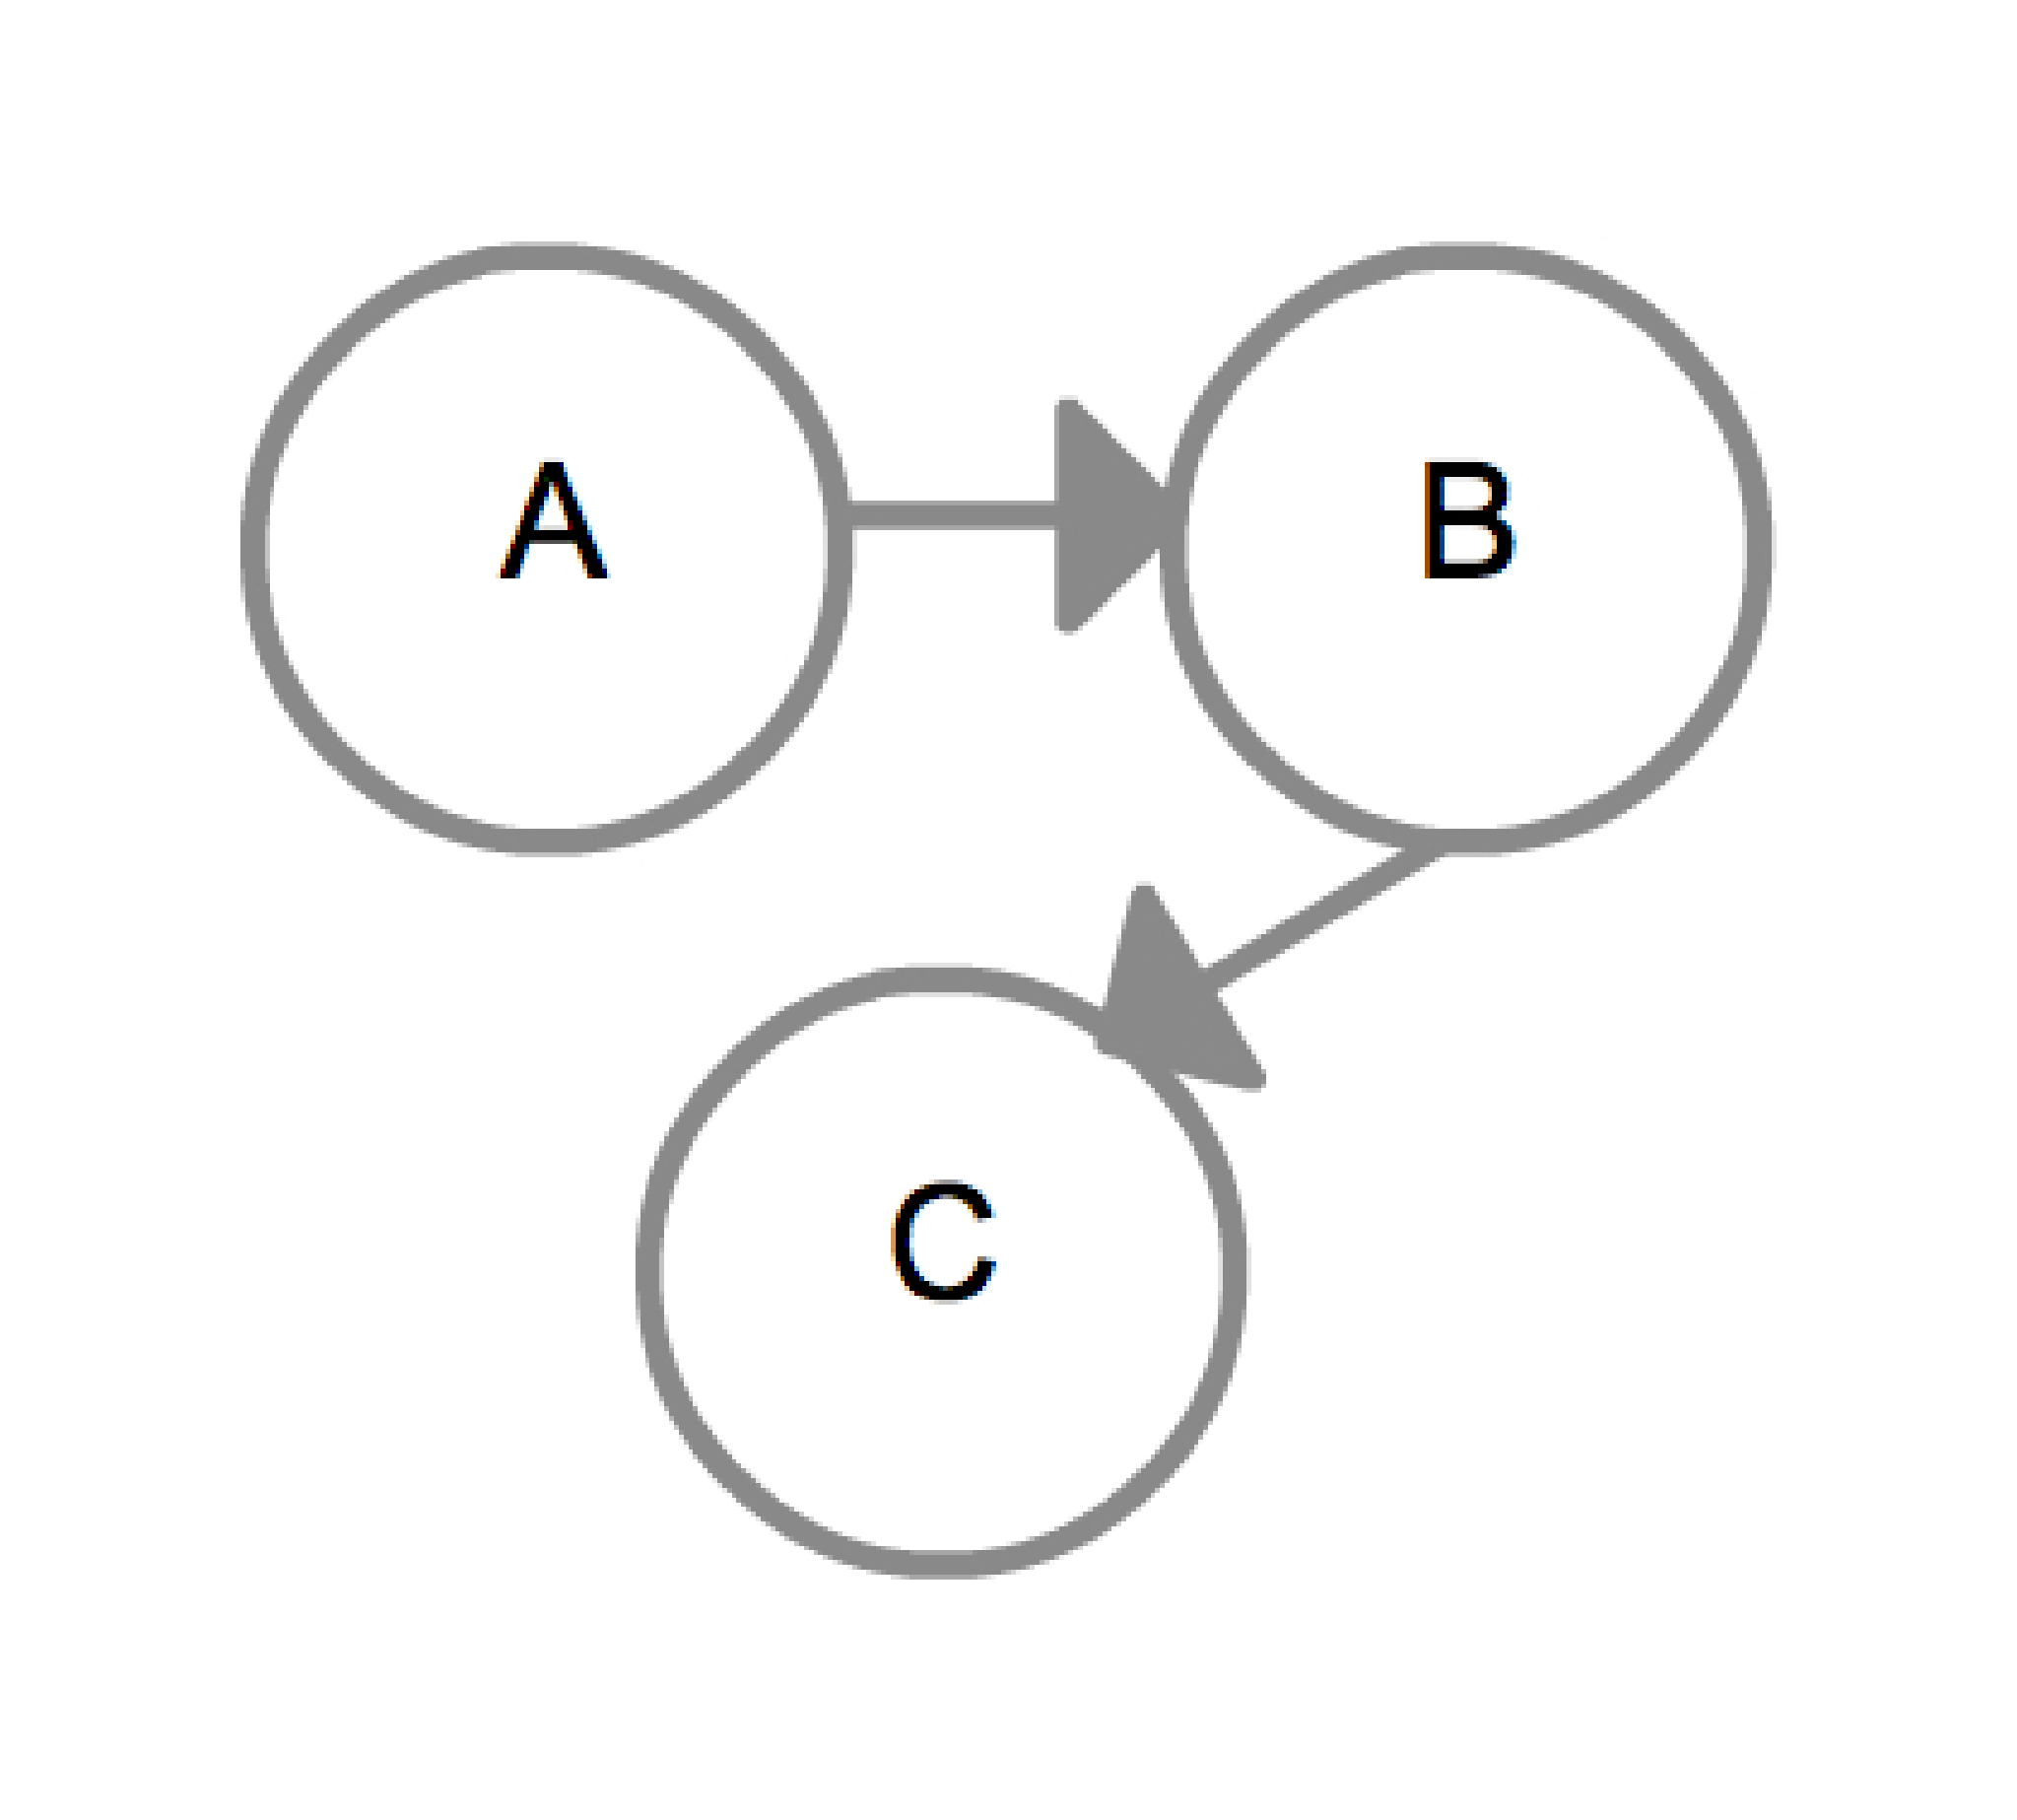
\includegraphics[scale=0.2]{DiGraph}
  %\caption{Demonstrates a directed graph}
  \label{fig:DiGraph}
}

Generally when we say graph, we mean undirected graph and will specify
directed graph or \emph{digraph}.

In a digraph, the number of incoming edges of $v$ is the in-degree or
$deg^-(v)$.  Similarly, the number of outgoing edges is the
out-degree or $deg^+(v)$.

In the above example:
%
\begin{align*}
deg^+(A) = deg^+(B) &= 1 \\
deg^-(B) = deg^-(C) &= 1 \\
deg^+(C) = deg^-(A) &= 0
\end{align*}

A \emph{simple graph} is a graph which contains no edges from any
vertex $v$ to itself $ (v,v) $, called loops.  A simple graph also
contains no multi-edges which connect more than two vertices.

A \emph{path} is a sequence of edges from vertex $u$ to vertex $v$.

Two vertices are said to be \emph{connected} if there exists a path
between them.  

A graph is said to be connected if for any two vertices, there exists
a path between them. An adjacent vertex is called a \emph{neighbour}.

A \emph{complete} graph is one in which every vertex is adjacent to
every other vertex.

A \emph{subgraph} is a graph consisting of a subset of the vertices
and edges in another graph.

A \emph{connected component} is a connected subgraph which does
not disconnect any adjacent vertices.  It should be easy to see that a
connected graph has exactly one connected component.

\section{Representation}

\subsection{Adjacency List}

One way to represent a graph is for every vertex, store a list of
neighbours.  For example:

{
  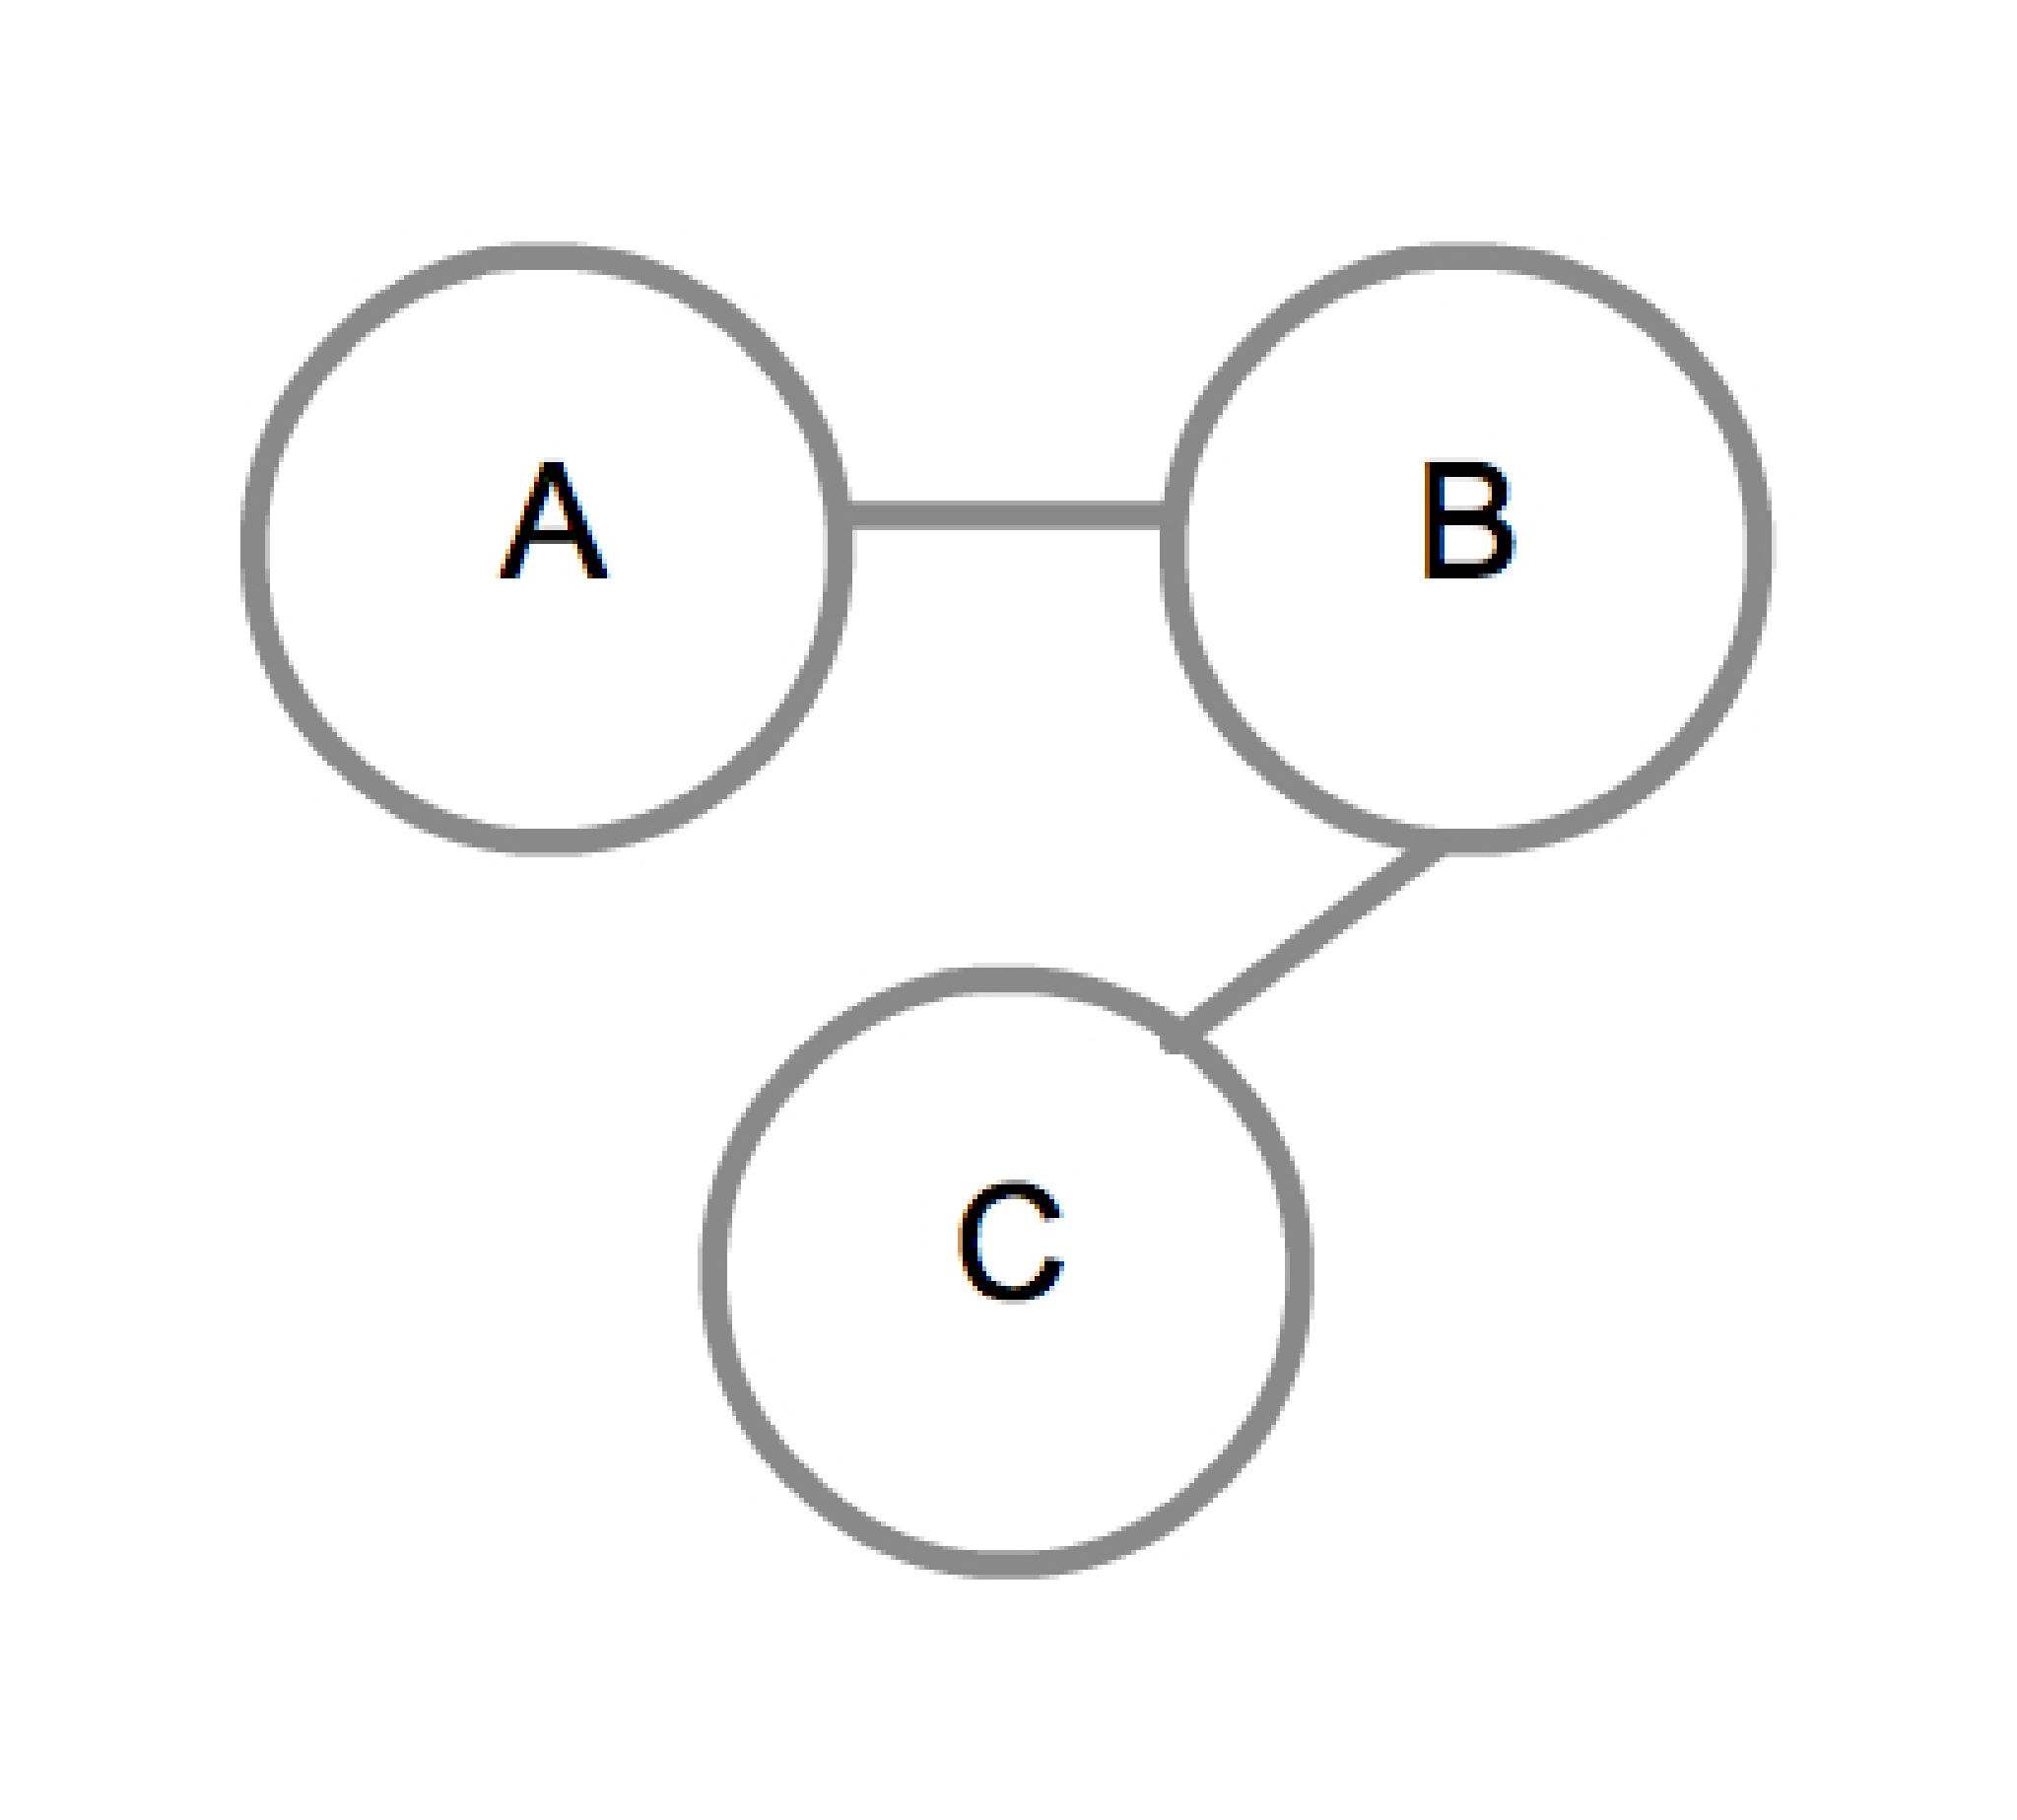
\includegraphics[scale=0.2]{SimpleGraph}
  %\caption{Demonstrates a simple graph}
  \label{fig:SimpleGraph}
}

can be represented:

{
  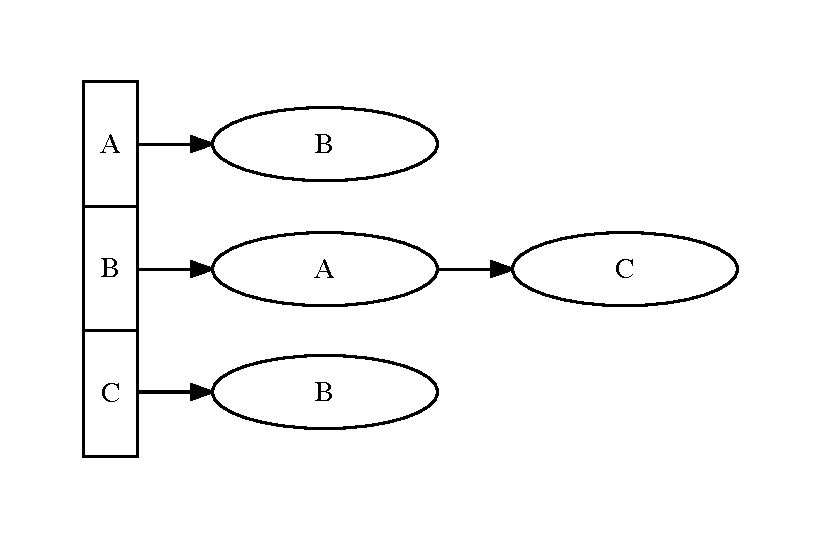
\includegraphics[scale=0.7]{AdjacencyList}
  %\caption{Demonstrates an adjacency list for a simple graph}
  \label{fig:AdjacencyList}
}

And

{
  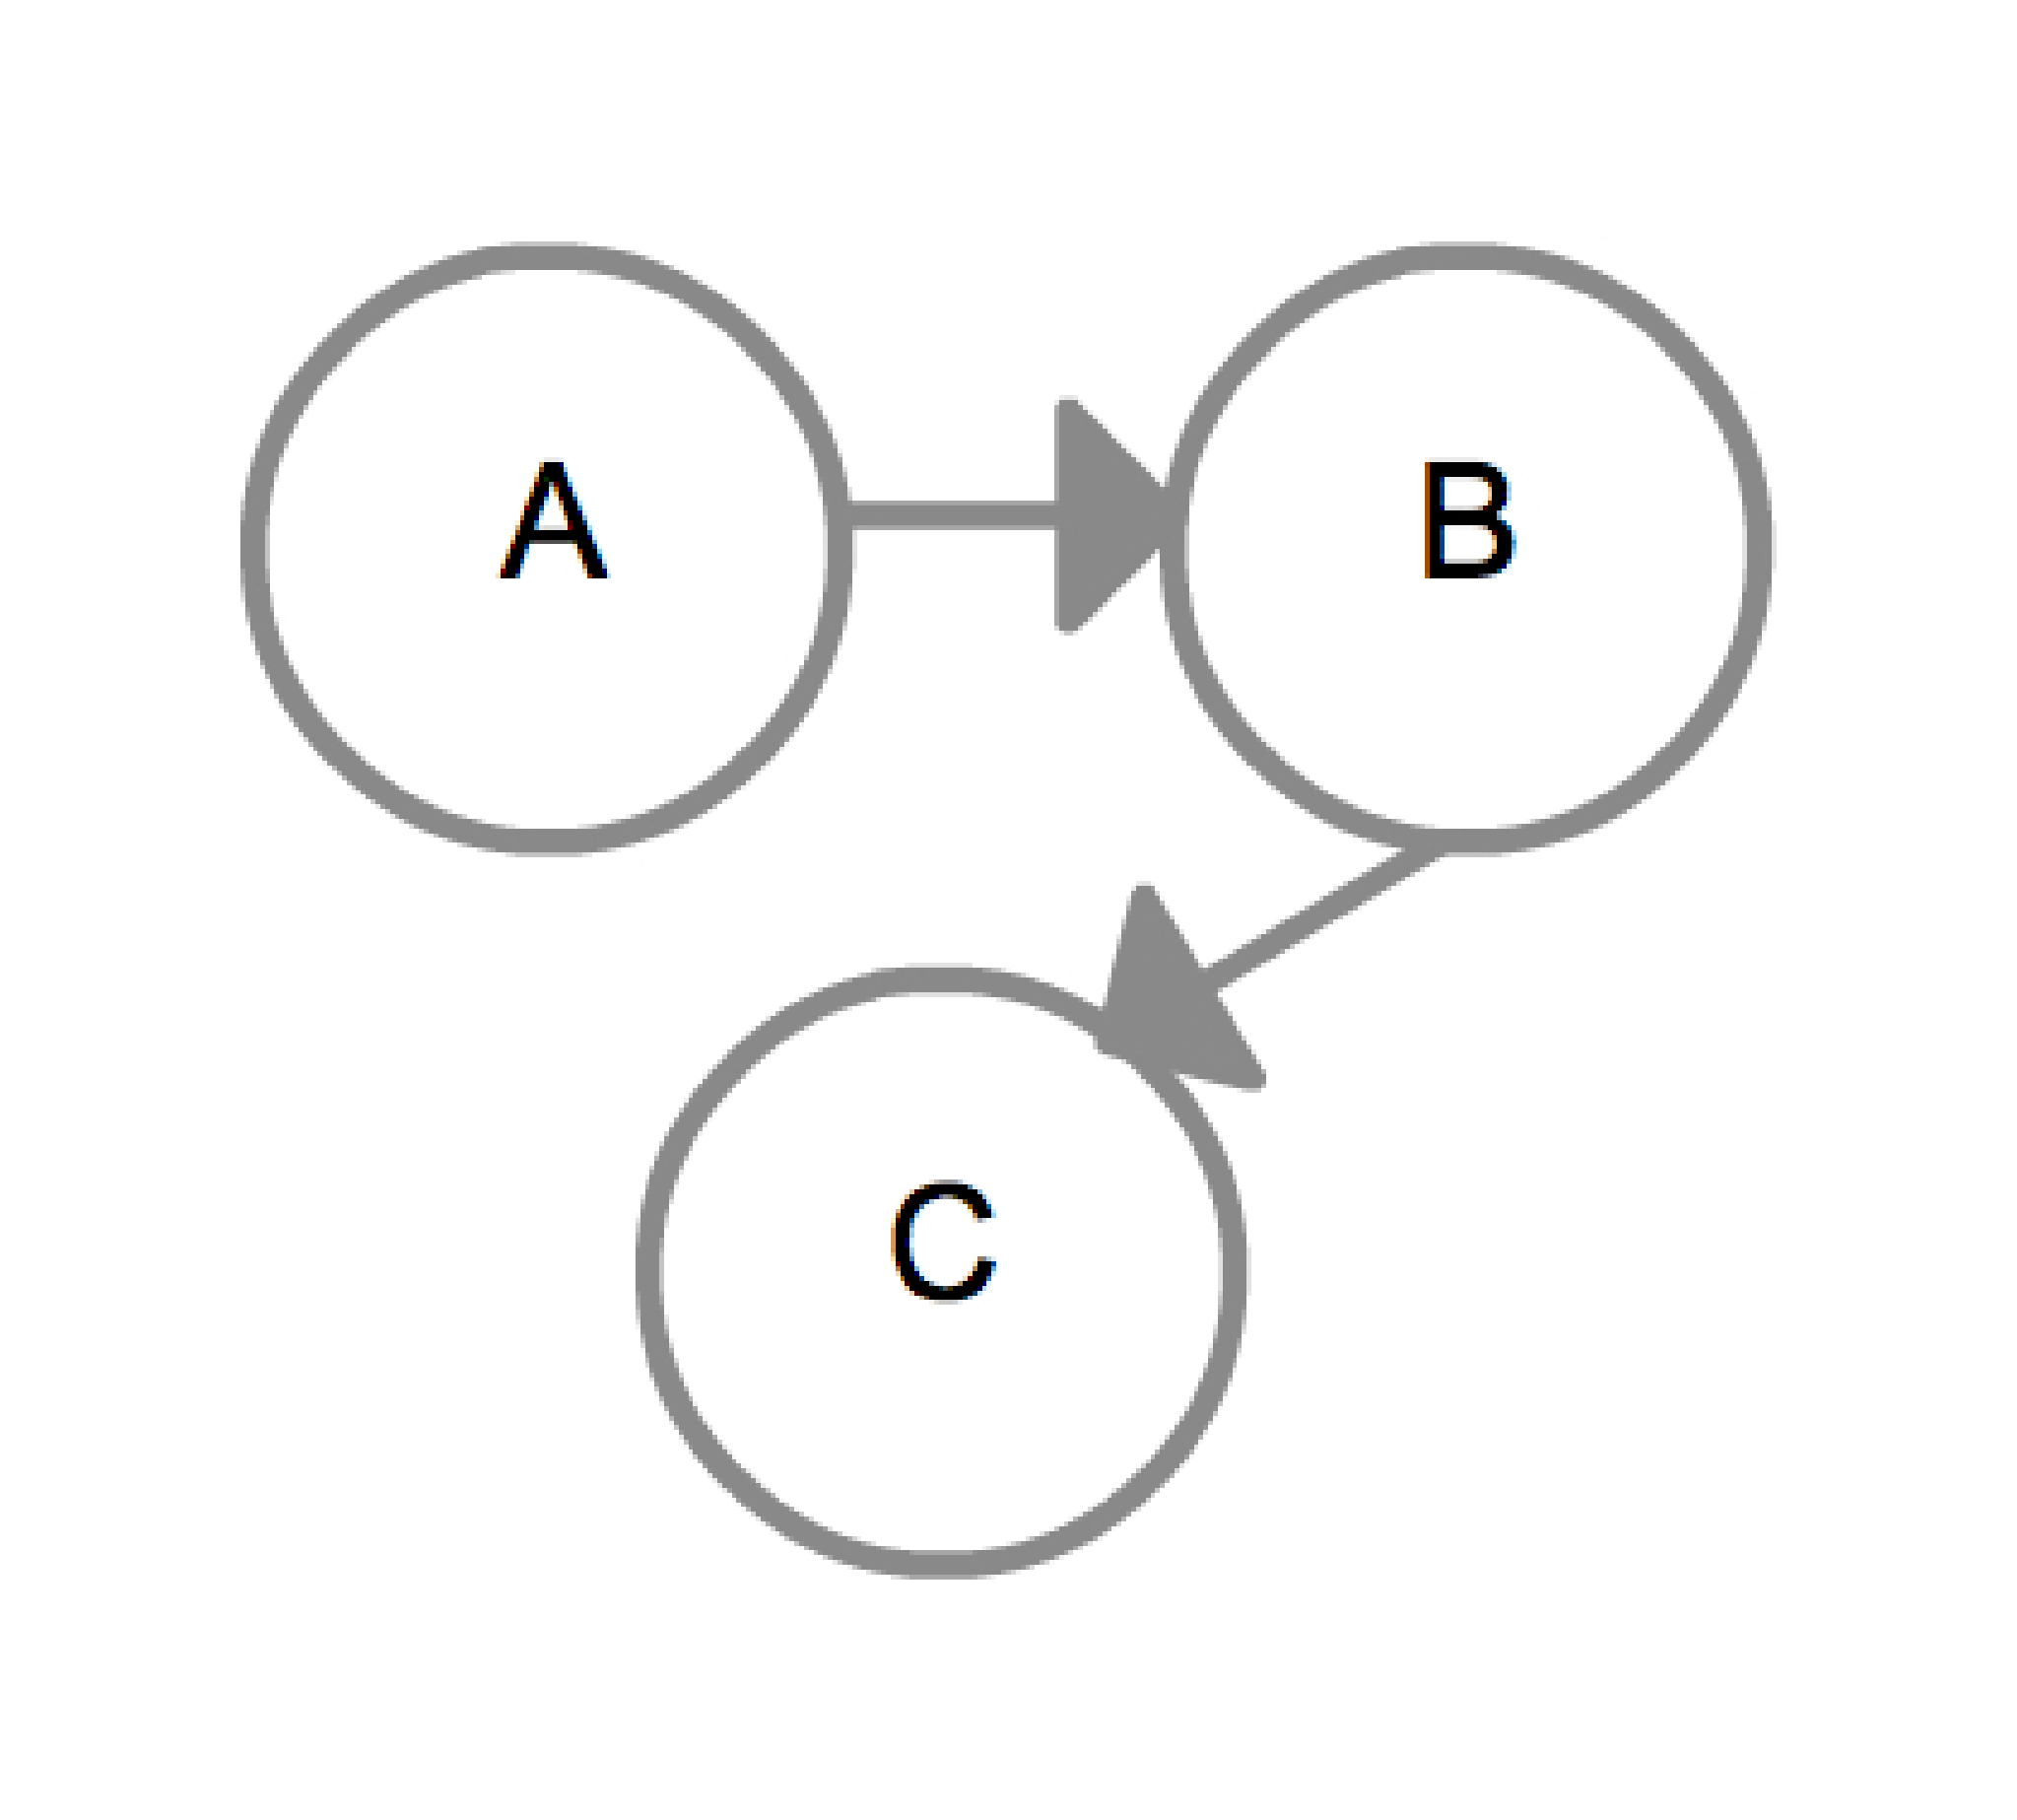
\includegraphics[scale=0.2]{DiGraph}
  %\caption{Demonstrates a directed graph}
  \label{fig:DiGraph}
}

can be represented:

{
  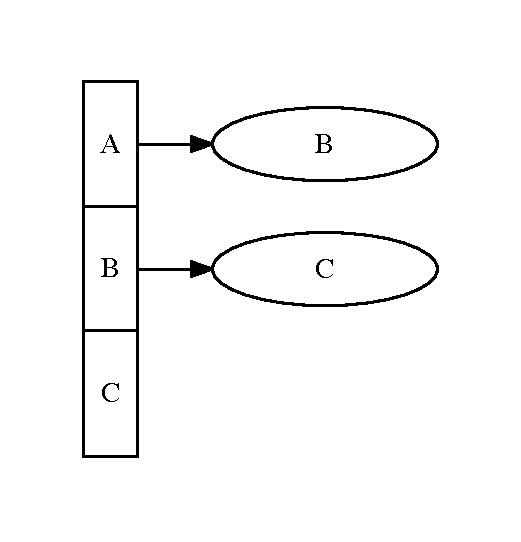
\includegraphics[scale=1.0]{AdjacencyListDigraph}
  %\caption{Demonstrates an adjacency list for a directed graph}
  \label{fig:AdjacencyListDigraph}
}

\subsection{Adjacency Matrix}

Another representation of a graph is as a square matrix with $n$ rows
and columns where the element at row $i$ and column $j$ is 1 if there
is an edge between $v_i$ and $v_j$ and 0 otherwise.  For example:

{
  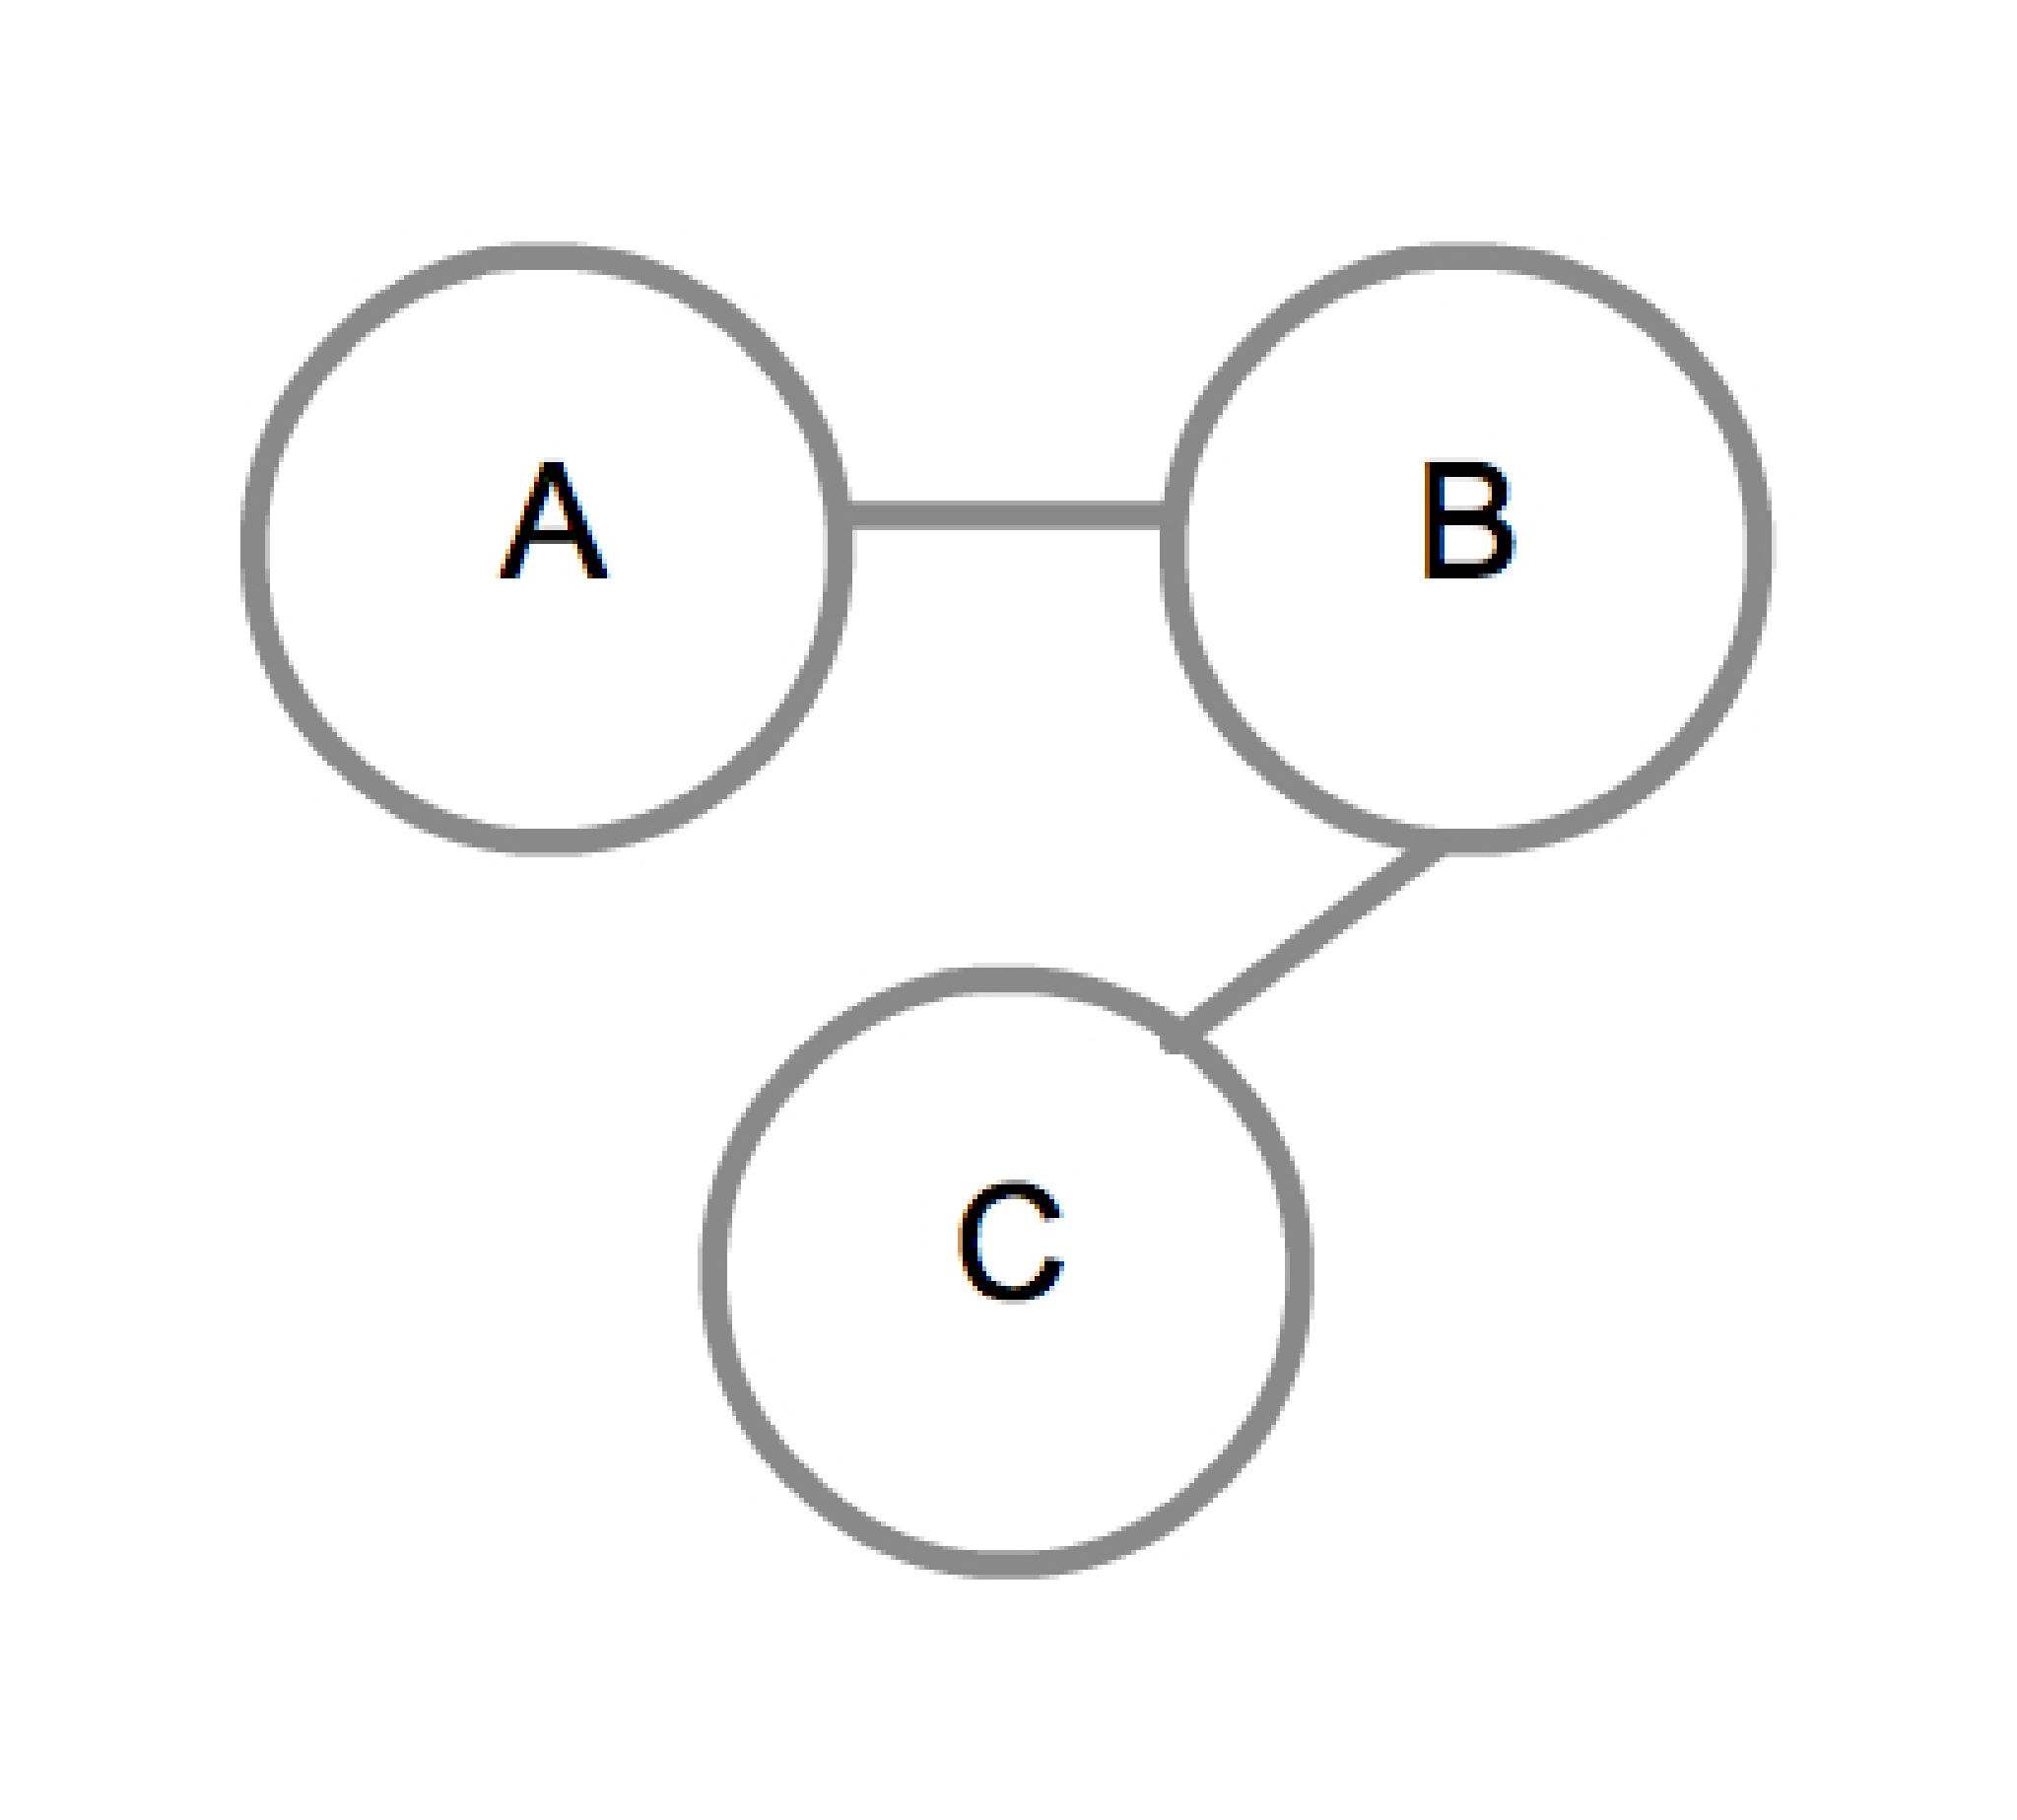
\includegraphics[scale=0.2]{SimpleGraph}
  %\caption{Demonstrates a simple graph}
  \label{fig:SimpleGraph}
}

can be represented

\[
\left[
\begin{array}{cccc}
  & a & b & c \\
a & 0 & 1 & 0 \\
b & 1 & 0 & 1 \\
c & 0 & 1 & 0
\end{array}
\right]
\]

As for directed graphs, row $i$ column $j$ is 1 if there exists an
edge $(v_i,v_j)$.  For example:

{
  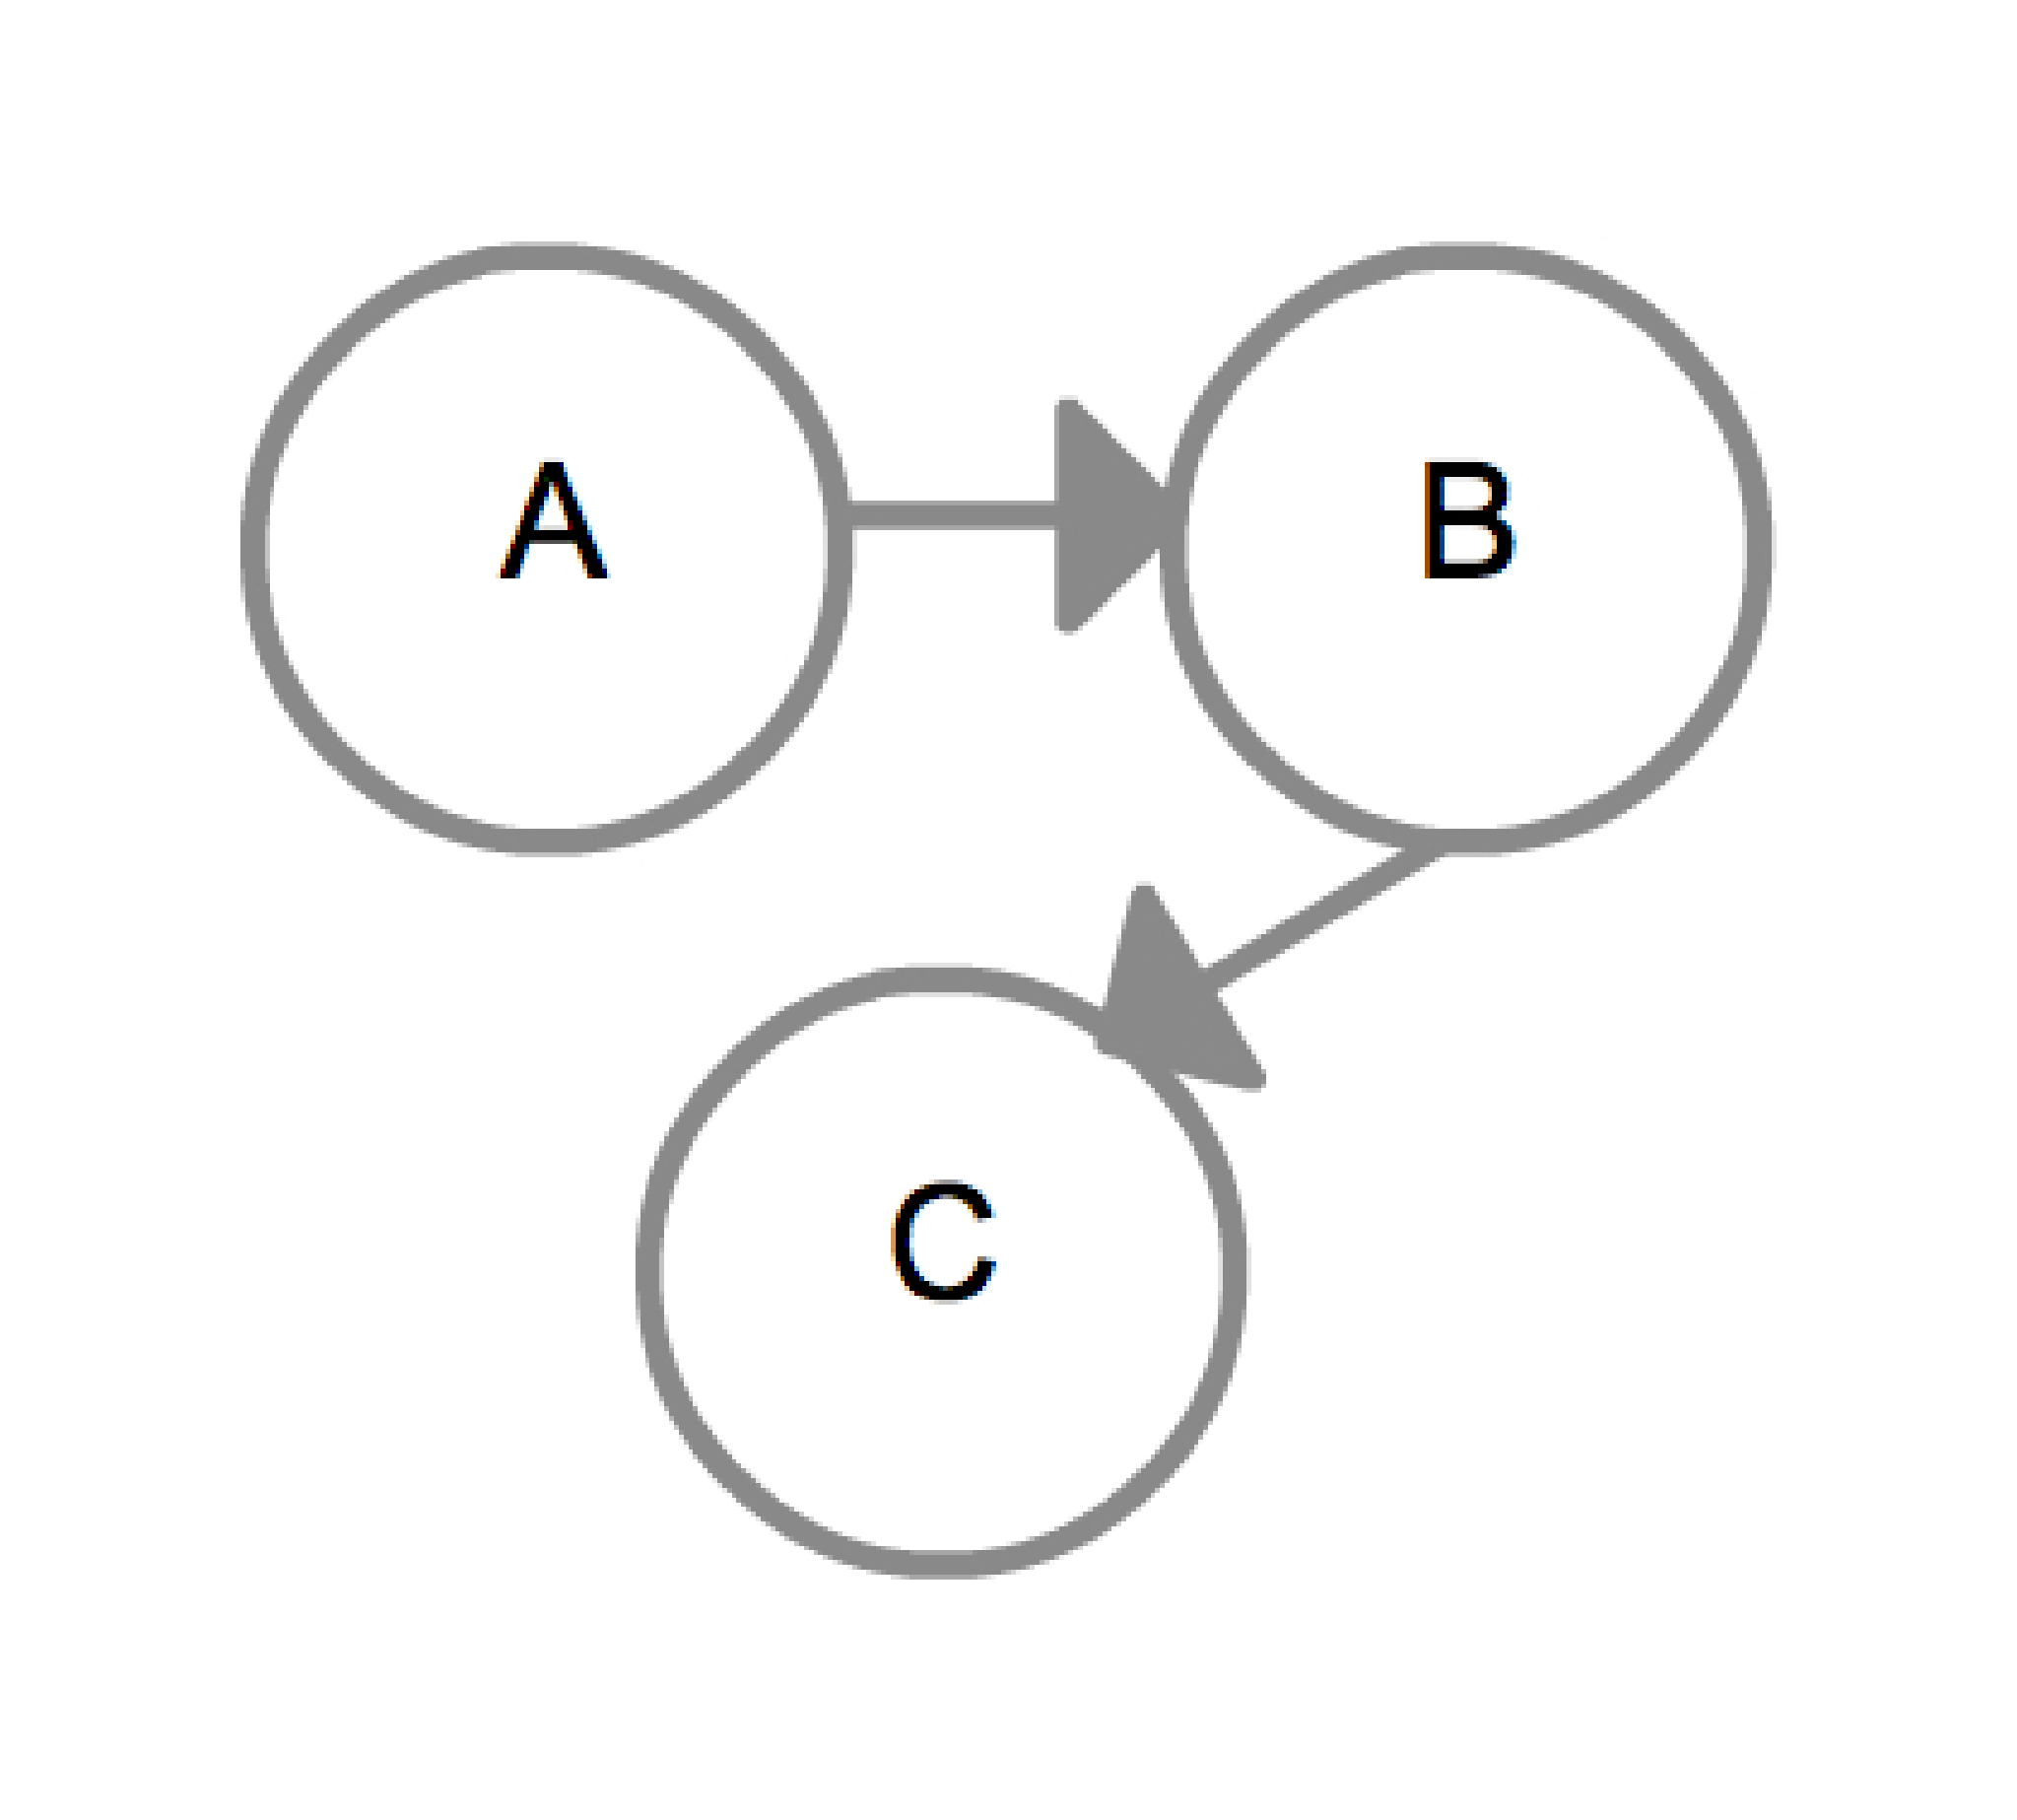
\includegraphics[scale=0.2]{DiGraph}
  %\caption{Demonstrates a directed graph}
  \label{fig:DiGraph}
}

can be represented

\[
\left[
\begin{array}{cccc}
  & a & b & c \\
a & 0 & 1 & 0 \\
b & 0 & 0 & 1 \\
c & 0 & 0 & 0
\end{array}
\right]
\]
